\section{引言}
模拟电路仿真(图\ref{fig:simulator-flowchart})
\cite{nagel1971computer,mccalla1971bias,Nagel:M382},经过在代数微分方程理论
\cite{estevez2000structural,kunkel2006differential,gunther2005modelling}、
器件建模\cite{chauhan2012bsim,ezaki2008physics,gildenblat2006psp}、
方程组构建\cite{hachtel1971sparse,ho1975modified,fijnvandraat2002time}、
方程组求解\cite{nastov2007fundamentals,najm2010circuit}、
硬件描述语言(HDL)\cite{verilog2014verilog,ieee2006ieee-1364-2005,
lemaitre2002adms,christen1999vhdl,pecheux2005vhdl}
等各领域的长期发展,已成为模拟电路 EDA 工具链中辅助验证和设计最重要的工具之一。
\begin{figure}[htpb]
  \centering
  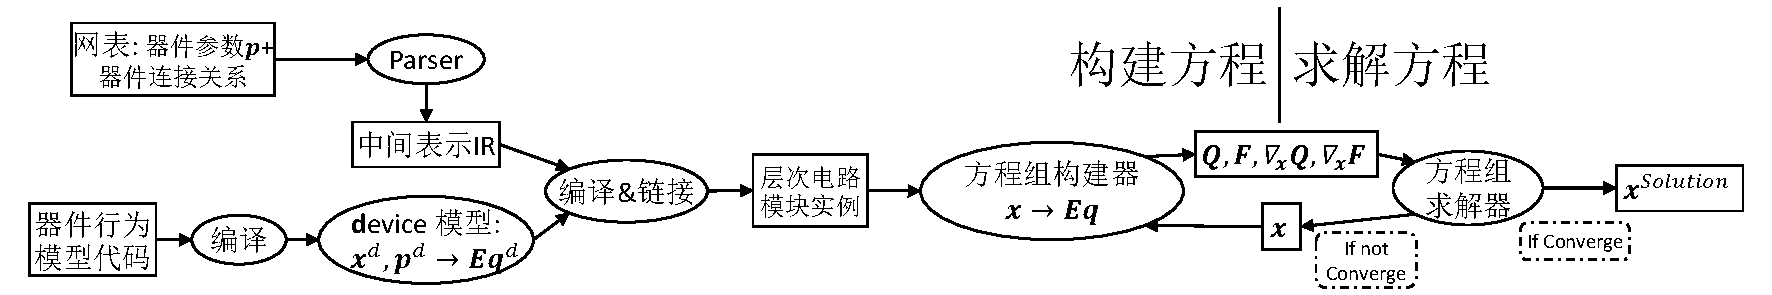
\includegraphics[width=1.0\textwidth]{fig/simulator-flowchart.pdf}
  \caption{仿真器内部流程图}
  \label{fig:simulator-flowchart}
\end{figure}
然而,当前主流 HDL 与仿真器对于复用粗粒度电路模块行为模型、引入多物理效应
以及在自动设计中应用梯度优化方法等方面的功能支持还有一些不便之处:
\begin{itemize}[partopsep=0pt,topsep=0pt,itemsep=0pt,parsep=0pt]
  \item
    器件及电路建模方面,HDL 常被用于实现器件行为模型,再编译
    \cite{lemaitre2002adms}为仿真器可调用的程序。 然而,% 引入器件 Aging 效应
    % 需借助 CMC-OMI\cite{CMC-OMI,velarde2019integration} 来修改模型参数;
    多端口电路行为建模常常需拆成两步:先做函数拟合,再表达成 HDL 实现,
    例如神经网络拟合\cite{meijer2001neural,zhang2017artificial}+HDL
    或 Volterra 多项式\cite{zhang2014large}+SPICE 网表
    等等\cite{zhang2019new,roymohapatra2019novel}。
  \item
    模拟电路设计\cite{razavi2002design,silveira1996g,jespers2009gm}
    自动化需考虑器件尺寸寻优,使电路多指标达到较优。
    在早期,研究者可借助参数敏感度分析使用梯度优化
    \cite{zhan2004optimization,agrawal2006circuit}求解。
    随着工艺及软件演进,更改设计变量需借助软件平台触发 Callback
    以修改模型参数,这导致用户无法获取变量的梯度信息,
    因此,新的研究热点转向了黑盒方法,如局部采样重构梯度
    \cite{huang2013efficient,nieuwoudt2005multi,peng2016efficient}、
    建立代理模型
    \cite{girardi2011analog,lyu2018batch,wang2014enabling,lyu2017efficient}
    或强化学习\cite{tang2018parametric}。
\end{itemize}
对上述现状,有一些模型编译、梯度获取方面的工作,例如 \citet{mahmutoglu2018new}
开发的 Verilog-AMS 编译器可使用 Matlab/Octave 运行,\citet{kuthe2020verilogae}
在编译 Verilog-AMS 电路模块时可获得更多方程及内部导数信息,
\citet{hu2020adjoint} 研究了瞬态仿真伴随方程的一种高效实现。
但是,这些工作均未考虑从方程组构建方法层面提供新的功能支持。

事实上,造成这些不便的一个重要原因是,
模拟 HDL 为同时支持结构信息与行为信息的表示,
包含了许多复杂乃至臃肿的功能,
例如模拟信号仿真所必须的自动微分、
建模可能用到的插值拟合\cite[Sec4.5.6,Sec9.21]{verilog2014verilog},
这两种信息的耦合导致模拟 HDL 既不易受益于其他语言及工具的开放生态,
也增加了开发模拟 EDA 工具的门槛。
此外,嵌套电路模块之间仅可传递不依赖于信号值的静态电路参数,
仿真运行时变量只能存在于模块内
(\cite[Sec3.4,Sec6]{verilog2014verilog},\cite[Sec4.10]{ieee2006ieee-1364-2005}),
% \cite[Sec3.4,Sec6; Sec4.10]{verilog2014verilog,ieee2006ieee-1364-2005},
这不利于粗粒度电路模型的复用与开发。

\paragraph{本文工作} 近年来,深度学习\cite{goodfellow2016deep}及
自动微分编程\cite{baydin2018automatic}等优秀工具的发展,
影响了科学计算中数据驱动的多尺度建模、反问题等许多研究
\cite{zhang2018deep,long2018pde,long2019pde}。
受此启发,本文提出了一种层次化(Hierarchical Circuit Simulation)
电路仿真\cite{fijnvandraat2002time,
ter1999numerical,mukherjee1999hierarchical,tcherniaev2003transistor}
中方程组构建器的计算图实现及对应的 JSON 网表与编译方法(图\ref{fig:flowchart}),
以统一的方式处理电路模块内外变量、设计变量、模型输入参数及相应的梯度。
本工作以电路模块作为计算图的基本计算单元,
支持使用 “JSON 网表定义等效电路分解 + SubModel 计算动态参数” 解耦表示电路模型:
(1)JSON 格式易解析,且其基本数据类型 “字典+列表” 已足以表示电路结构信息;
(2)SubModel 实现时可借助相应工具如 Julia\cite{Bezanson_Julia_A_fresh_2017}
的自动微分能力; 这种表示可降低电路模型开发难度并增强仿真工具的梯度获取能力。
\begin{figure}[htpb]
  \centering
  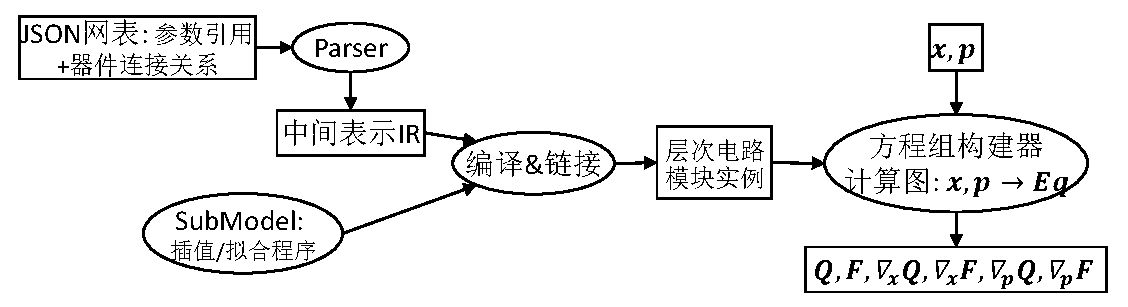
\includegraphics[width=0.7\textwidth]{fig/flowchart.pdf}
  \caption{计算图及JSON网表编译}
  \label{fig:flowchart}
\end{figure}

类似于编程语言的函数的定义、编译、表示、执行
\cite{aho2007compilers,muchnick1997advanced,appel2004modern},
Sec \ref{sec:Joanna} 详细讨论了计算图中电路模块结构信息的处理:
模块定义(网表)、解析与编译、模块实例的数据结构、
执行引擎(计算图,图\ref{fig:equations-system-constructor}),
此外,Sec \ref{subsec:EvalCompositeSubCkt} 还介绍了如何定义和使用 SubModel
计算内部变量作为动态参数以提供电路模块的行为信息。
Sec \ref{sec:applications} 介绍了两个应用示例,
包括器件模型、多 PVT 下联合求解 DC,AC 分析与器件尺寸寻优。
